\newpage
\section{Standard di qualità}
Il team di sviluppo prende come riferimento per gli obiettivi di qualità del prodotto i seguenti standard.

In questa appendice verranno descritti gli standard adottati, nelle \NdP\D invece come questi saranno applicati e nel \PdQ~gli obiettivi che il team di sviluppo si è dato per seguendo gli standard scelti.

	\subsection{ISO/IEC 15504 (SPICE)}
	Lo standard ISO/IEC 15504 è stato creato per unire in un unico standard le caratteristiche principali di \gloss{CMMI} e \gloss{SPY}; entrambi standard riguardanti la qualità di processi software.
	
	ISO/IEC 15504 è chiamato anche SPICE come acronimo di \textit{Software Process Improvement and Capability Determination}, dando importanza al termine \textit{Capability} inteso come la capacità di un processo di essere cognitivamente capace di raggiungere il suo scopo. Un processo con un'alta \textit{capability} è osservato da tutto il team di sviluppo in modo disciplinato e sistematico, al contrario il processo viene effettuato in modo opportunistico e disorganizzato.
	
	SPICE mette a disposizione una metrica per valutare diversi attributi per ogni processo ed assegna un valore quantitativo ad ognuno di questi in modo tale da rendere esplicito come poter migliorare tale processo. Ogni valutazione in questo modo può essere ripetibile, oggettiva e comparabile.
	
	I processi vengono classificati in:
	
	\begin{itemize}
		\item \textbf{Customer/Supplier}
		\item \textbf{Engineering}
		\item \textbf{Support}
		\item \textbf{Management}
		\item \textbf{Organization}
	\end{itemize}
	
	Gli attributi per valutare i processi classificati per livelli sono:
	
	\begin{itemize}
		\item \textbf{0 Incomplete}: il processo è caotico perché con risultati e performance incomplete;
	
		\item \textbf{1 Performed}: il processo inizia ad essere eseguito mettendo a disposizione degli input ed output.
		
		Attributi:
		
		\begin{itemize}
			\item \textbf{Execution of processes}: indica quantitativamente il numero di obiettivi raggiunti;
		\end{itemize}
	
		\item \textbf{2 Managed}: le responsabilità e la gestione del progetto sono definite.
		
		Attributi:
		
		\begin{itemize}
			\item \textbf{Management of process}: indica quanto sono organizzati gli obiettivi fissati;
			\item \textbf{Management of products}: indica quanto sono organizzati o gestiti i prodotti rilasciati;
		\end{itemize}
	
		\item \textbf{3 Established}: il processo è pronto per diventare un processo standard ed essere rilasciato.
		
		Attributi:
		
		\begin{itemize}
			\item \textbf{Definition of process}: indica quanto il processo aderisce agli standard;
			\item \textbf{Distribution of process}: indica in che misura il processo possa essere rilasciato potendo restituire sempre lo stesso risultato;
		\end{itemize}
	
		\item \textbf{4 Predictable}: il processo è in grado di essere sottoposto a metriche e valutazioni quantitative. Spesso i risultati sono predicibili.
		
		Attributi:
		
		\begin{itemize}
			\item \textbf{Measurements of process}: indica quanto le metriche possono essere applicate al processo;
			\item \textbf{Controll of process}: indica quanto i risultati delle valutazioni siano predicibili;
		\end{itemize}
	
		\item \textbf{5 Optimizing}: il processo attua miglioramenti qualitativi e quantitativi.
		
		Attributi:
		
		\begin{itemize}
			\item \textbf{Process innovation}: indica quanto i cambiamenti attuati nel processo risultino innovativi e positivi grazie ad una fase di analisi;
			\item \textbf{Optimization of process}: indica quanto la curva di miglioramento del processo sia lineare;
		\end{itemize}
	\end{itemize}
	
	Ad ogni attributo viene data una valutazione assegnata in base alla percentuale di soddisfacimento dell'attributo:
	
	\begin{itemize}
		\item \textbf{N}: il processo non è implementato e non svolge niente di significativo (0\%-15\%);
		\item \textbf{P}: il processo è parzialmente implementato (15\%-50\%);
		\item \textbf{L}: il processo è largamente implementato (50\%-85\%);
		\item \textbf{F}: il processo è completamente implementato (85\%-100\%); 
	\end{itemize}
	
	\begin{table}[h]
	\centering
	\begin{tabular}{ccccc}
		
		\toprule
		\multirow{2}{*}{Attributi} & \multicolumn{4}{c}{Valutazioni}\\
		\cmidrule(lr){2-5} & N & P & L & F\\
		\midrule Execution of processes & \multicolumn{4}{c}{[0-1]}\\
		\midrule Management of process & \multicolumn{4}{c}{\multirow{2}{*}{[1-2]}}\\
		Management of products\\
		\midrule Definition of process & \multicolumn{4}{c}{\multirow{2}{*}{[2-3]}}\\
		Distribution of process\\
		\midrule Measurements of process & \multicolumn{4}{c}{\multirow{2}{*}{[3-4]}}\\
		Controll of process\\
		\midrule Process innovation & \multicolumn{4}{c}{\multirow{2}{*}{[4-5]}}\\
		Optimization of process\\
		\bottomrule
		
		
		
	\end{tabular}
	\label{tab:spice}
	\caption{Schema degli attributi di ISO/IEC 15504}
	\end{table}

	\subsection{IEC/ISO 9126:2001}
	ISO/IEC 9126 è uno standard inerente alla qualità del software. Esso è strutturato in modo tale che si possa migliorare l'insieme dei processi.
	
	La sua struttura prevede tre tipi di qualità, ognuna delle quali possiede determinate caratteristiche:
	
	\begin{itemize}
		\item \textbf{Qualità interna}: misura la qualità di chi causa l'esecuzione del prodotto, in questo caso parliamo del codice sorgente a chi si possono assegnare diverse metriche attraverso l'analisi statica che ne stabiliscono poi la portabilità e la manutenibilità.
		
		Gli attributi ad essa assegnati sono:
		
		\begin{itemize}
			\item \textbf{Manutenibilità}
			\item \textbf{Portabilità}
		\end{itemize}
	
		\item \textbf{Qualità esterna}: misura attraverso l'analisi dinamica quanto l'esecuzione del prodotto rispetti gli obiettivi prefissati.
		
		Gli attributi ad essa assegnati sono:
		
			\begin{itemize}
			\item \textbf{Funzionalità}
			\item \textbf{Efficienza}
			\item \textbf{Affidabilità}
			\item \textbf{Usabilità}
		\end{itemize}
	
		\item \textbf{Qualità in uso}: definisce le metriche del prodotto rilasciato ed usato dal cliente che ne misurerà la qualità.
		
		Gli attributi ad essa assegnati sono:
		
		\begin{itemize}
			\item \textbf{Efficacia}
			\item \textbf{Produttività}
			\item \textbf{Soddisfazione}
			\item \textbf{Safety}
		\end{itemize}
	\end{itemize}

		\subsubsection{Descrizione degli attributi della Qualità interna e della Qualità esterna}
		\begin{itemize}
			\item \textbf{Manutenibilità}: il software nel corso delle sue revisioni deve essere facilmente modificabile.
			
			Nello specifico si prevede:
			
			\begin{itemize}
				\item \textbf{Analizzabilità}: prevedere una lettura del codice fruibile;
				\item \textbf{Modificabilità}: poter capire subito dove applicare la modifica;
				\item \textbf{Stabilità}: evitare effetti indesiderati dopo le modifiche;
				\item \textbf{Testabilità}: poter creare facilmente dei test su tutto il codice;
			\end{itemize}
		
			\item \textbf{Portabilità}: il software dovrebbe poter essere eseguito in più ambienti.
			
			Nello specifico si prevede:
			
			\begin{itemize}
				\item \textbf{Adattabilità}: potersi adattare automaticamente ai vari ambienti:
				\item \textbf{Installabilità}: la sua fase d'installazione dovrebbe essere semplice;
				\item \textbf{Conformità}: il software deve sapere coesistere con le altre applicazioni;
				\item \textbf{Sostiuibilità}: essere capace di sostituire un software con gli stessi scopi;
			\end{itemize}
		
			\item \textbf{Funzionalità}: il software deve mettere a disposizione le funzionalità richieste in rapporto all'ambinete d'esecuzione.
			
			Nello specifico si prevede:
			
			\begin{itemize}
				\item \textbf{Appropriatezza}: le funzionalità del software sono appropriate ai requisiti richiesti;
				\item \textbf{Accuratezza}: in che misura le funzionalità aderiscono ai requisiti richiesti;
				\item \textbf{Interoperabilità}: la capacità di interagire coi sistemi specificati;
				\item \textbf{Security}: preteggere le informazioni da agenti esterni;
			\end{itemize}
		
			\item \textbf{Efficienza}: misura della capacità di raggiungere gli obiettivi stabiliti cercando di usare meno risorse possibili.
			
			Nello specifico si prevede:
			
			\begin{itemize}
				\item \textbf{Nel tempo}: poter dare risposte in un tempo di scadenza appropriato;
				\item \textbf{Nello spazio}: utilizzo del minor numero di risorse; 
			\end{itemize}
		
			\item \textbf{Affidabilità}: il software deve mantenere le specifiche richieste senza inconvenienti.
			
			Nello specifico si prevede:
			
			\begin{itemize}
				\item \textbf{Maturità}: indica il livello minimo delle parti del prodotto che si rivela poi essere il livello di qualità dell'intero prodotto;
				\item \textbf{Robustezza}: la capacità di saper reagire agli errori;
				\item \textbf{Recuperabilità}: poter tornare alla versione precedente del software in modo semplice;
			\end{itemize}
		
			\item \textbf{Usabilità}: il software deve poter essere compreso fin da subito, dunque semplice ed immediato nell'utilizzo e comprensione.
			
			Nello specifico si prevede:
			
			\begin{itemize}
				\item \textbf{Comprensibilità}: il significato delle funzionalità deve essere compreso il prima possibile dall'utente;
				\item \textbf{Apprendibilità}: capacità di saper usare le funzionalità disponibili;
				\item \textbf{Operabilità}: capacità dell'utente di usare e controllare il software;
				\item \textbf{Attrattiva}: il risultato risulta attraente all'utente; 
			\end{itemize}
		\end{itemize}
	
		\subsubsection{Descrizione degli attributi della Qualità in uso}
		\begin{itemize}
			\item \textbf{Efficacia}: misura della capacità di riuscire a raggiungere i compiti fissati. Essa si calcola
			in base al grado di raggiungimento degli obiettivi;
			\item \textbf{Produttività}: intesa come $ \frac{\text{unità di prodotto realizzato}}{\text{unità di risorse utilizzate}} $;
			\item \textbf{Soddisfazione}: il software soddisfa l'utente;
			\item \textbf{Safety}: il software deve possedere adeguati livelli di sicurezza per il tipo di utente che ne usufruisce;
		\end{itemize}
	
	\begin{figure}[h]
		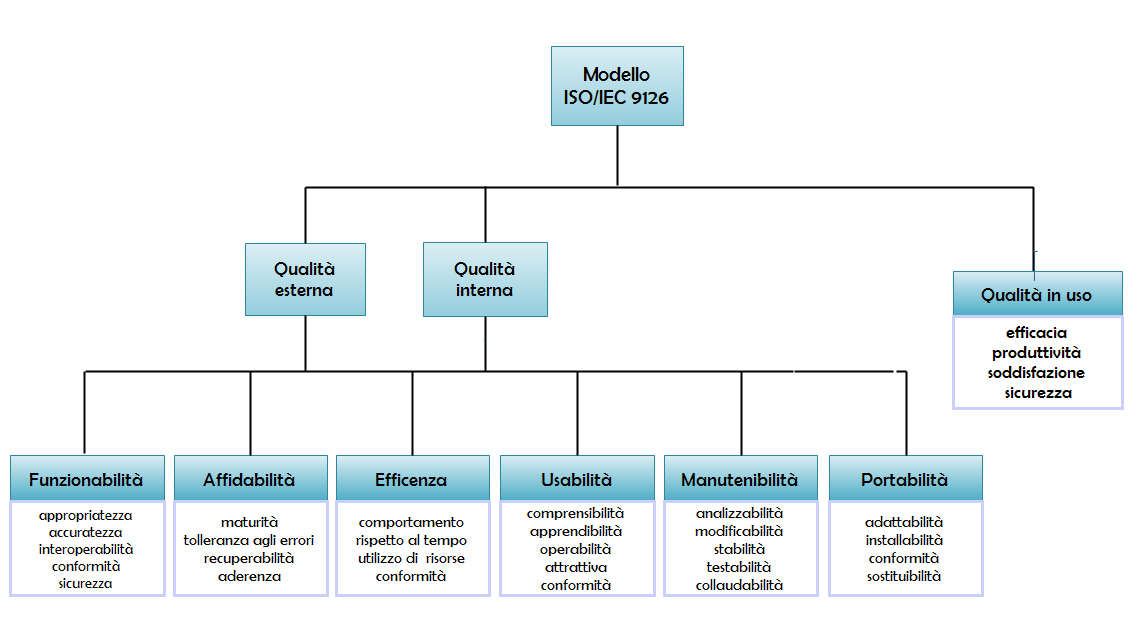
\includegraphics[width=\textwidth]{img/ISO9126.png}
		\label{fig:iso9126}
		\caption[Schema ISO 9126]{Schema ISO 9126 (tratto da Wikipedia)}
	\end{figure}

	
	
	\begin{figure}[h]
		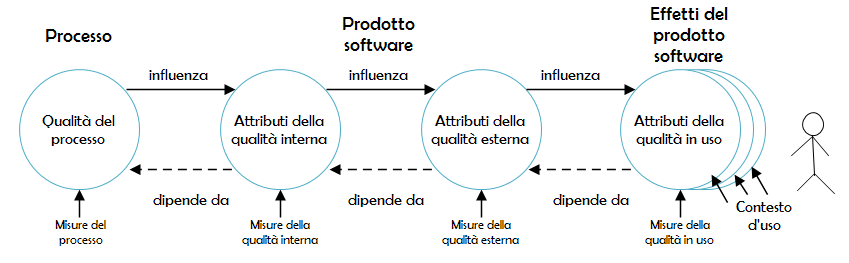
\includegraphics[width=\textwidth]{img/Ciclo_di_vita_9126.png}
		\label{fig:ciclo_di_vita}
		\caption[Ciclo di vita con l'ISO 0126]{Ciclo di vita applicando l'ISO 9126 (tratto da Wikipedia)}
	\end{figure}